





\section{Experiments}

\subsection{Experimental Setup}
\label{subsec:setup}

\subsubsection{Training Datasets.}

We train \ours{} on a heterogeneous mixture of omni-modal retrieval pairs that cover diverse modality compositions.
In particular, the training data include:
(1) text-only contrastive pairs from BGE-m3~\cite{bge-m3};
(2) text--image pairs from the MMEB-V1 training set~\cite{MMEB} and PixMo-Docs~\cite{PixMo};
(3) text--video retrieval pairs from MSR-VTT~\cite{MSR-VTT} and the MMEB-V2 training set~\cite{MMEB-v2};
(4) text--audio retrieval pairs from AudioCaps~\cite{AudioCaps};
(5) visual-document retrieval pairs from MMEB-V2~\cite{MMEB-v2}.
Overall, this mixture exposes the model to queries/ targets that are uni-modal, bi-modal, or composed of multiple modalities, which is critical for learning a unified omni-modal embedding space.

\subsubsection{Implementation Details.}
\label{subsubsec:imple_dets}

We adopt Qwen2.5-Omni~\cite{Qwen2.5-Omni} as the VLM backbone and fine-tune it with LoRA~\cite{lora} for parameter-efficient adaptation.
We set the maximum sequence length to 512 tokens for both queries and targets, and train for one epoch with a learning rate of $1\times 10^{-4}$ and a warmup ratio of 0.005.
Training is performed on 8 H100 GPUs with a per-device batch size of 20 and gradient accumulation of 2. 
For each dataset, we use two dataset-provided hard negatives per query.

For our method-specific components, we initialize the trainable modality scaling vector $\boldsymbol{\tau}$ to 0.02.
After training, the learned temperatures are
$\boldsymbol{\tau}=[0.0130,\,0.0127,\,0.0219,\,0.0223]$
for $\{\texttt{T},\texttt{I},\texttt{A},\texttt{V}\}$, respectively.
We set the debiasing coefficient $\gamma_{+} = 0.1$, $\rho_{\mathrm{init}}=0.1$, $\rho_{\mathrm{final}}=0.5$, and use $t_0=4000$ warmup steps before increasing hardness.
For batch whitening and covariance alignment, we set $\lambda_{\mathrm{coral}}=0.05$.
We report the settings of \ours{}-7B.
More details are in Appendix~\ref{app:impl_more}.

\subsubsection{Evaluation.}

We evaluate \ours{} on two benchmarks.
First, we use \textbf{MMEB-V2}~\cite{MMEB-v2}, a large-scale multimodal embedding benchmark covering \emph{text, image, video, and visual documents}.
It contains \textbf{9 meta-tasks and 78 tasks} spanning diverse categories such as retrieval, classification, question answering, and visual document retrieval.
Following the MMEB-V2 protocol, we use Hit@1 as the primary metric for image/video tasks and report NDCG@5 for visual-document tasks.
Second, we evaluate audio retrieval on \textbf{AudioCaps}~\cite{AudioCaps}, which contains about 4.4K text--audio pairs.
We report Recall@1, \ie, the fraction of text queries whose matched audio is ranked at the top.



\begin{table}[t]
\centering
\small
\caption{Overall results on AudioCaps.
We only include \textit{omni-modal} embedding models that are trained with audio data.
``$\ddag$'' denotes our model outperforms all baselines significantly in paired t-test at $p<0.05$ level (with Bonferroni correction).
}\label{tab:audiocaps-overall}
\begin{tabular}{
p{0.52\linewidth}
>{\centering\arraybackslash}p{0.12\linewidth}
>{\centering\arraybackslash}p{0.20\linewidth}
}
\toprule
Model & Size & Recall@1 \\
\midrule
\multicolumn{3}{l}{\textit{\textbf{Baselines}}} \\
Tevatron-Omni              & 7B  & 34.0 \\
LCO-EMB                    & 7B  & 24.2 \\
Omni-Embed-Nemotron        & 3B  & 20.5 \\
\midrule
\multicolumn{3}{l}{\textit{\textbf{Ours}}} \\
\ours{}-3B & 3B & 34.3 \\
\ours{}-7B & 7B & \textbf{37.7}$^\ddag$ \\
\bottomrule
\end{tabular}
\end{table}




\subsection{Overall Results}

Table~\ref{tab:mmeb-v2-overall} reports overall performance on \textbf{MMEB-V2}, and Table~\ref{tab:audiocaps-overall} reports \textbf{AudioCaps} text--audio retrieval results.
\ours{} outperforms strong bi-modal and omni-modal baselines on both benchmarks, supporting the effectiveness of our framework.

We highlight three observations:
(1)~\textbf{Broad gains across modalities and tasks.}
On MMEB-V2, \ours{} improves image/video retrieval and also yields clear gains on the visual-document retrieval subset, suggesting that explicit alignment remains beneficial under heterogeneous, long-form visual inputs.
(2)~\textbf{Improved audio retrieval.}
On AudioCaps, \ours{}-7B achieves higher Recall@1 than omni-modal baselines, indicating that our alignment components generalize beyond vision-language and improve the stability of audio embeddings.
(3)~\textbf{Scaling with model size.}
The alignment gains grow when scaling from 3B to 7B (All: $+1.1$ vs.\ $+2.0$), suggesting that explicit alignment is complementary to model scaling.





\subsection{Ablation Study}
\label{sec:ablation}

\begin{table}[!t]
    \centering
    \small
    \caption{Ablation of \ours{}.
We remove one component at a time from the full model and report results on MMEB-V2 and AudioCaps.
}\label{tab:ablation}
%    \setlength{\tabcolsep}{3.5pt}
%\setlength{\extrarowheight}{1.1pt}
    \begin{tabular}{
p{0.5\linewidth} @{}cc
%*{2}{>{\centering\arraybackslash}p{0.18\linewidth}}
} 
    \toprule
    Model & MMEB-V2 & AudioCaps \\
    \midrule
    \ours{}-7B & \textbf{66.4} & \textbf{37.7} \\
    \midrule
    \quad w/o. Modality-aware Temp. & 65.7 & 36.6 \\
    \quad w/o. Curriculum Schedule & 65.7 & 36.7 \\
    \quad w/o. DCL (w/ Curriculum)  & 66.1 & 37.0 \\
    \quad w/o. Whitening \& CORAL   & 65.9 & 36.3 \\
    \bottomrule
    \end{tabular}
%    \vspace{-0.15cm}    
\end{table}


To understand the contribution of each component in \ours{}, we conduct ablation studies by removing one design choice at a time while keeping all other settings fixed.
We report results on MMEB-V2 and AudioCaps in Table~\ref{tab:ablation}.
Overall, removing any component degrades performance, indicating that the proposed techniques are complementary.

\noindent\textbf{Modality-aware Temperature Calibration.}
Disabling modality-aware temperature calibration (\ie, using a single global temperature of 0.02, matching the initialization of $\boldsymbol{\tau}$) causes a clear performance drop.
This suggests that calibrating modality-dependent logit sharpness stabilizes contrastive optimization under mixed omni-modal batches.

\noindent\textbf{Controllable Negative Curriculum.}
We ablate the negative curriculum by (i) removing the curriculum schedule and using a fixed threshold 0.3, or (ii) removing DCL while keeping curriculum.
Both variants underperform \ours{}, indicating that progressively increasing negative hardness helps avoid unstable early training while improving fine-grained discrimination later.
We further observe additional degradation when removing DCL, suggesting that debiasing is important when hard-negative selection amplifies false-negative bias.

\noindent\textbf{Batch Whitening and Covariance Alignment.}
Removing whitening and the covariance regularizer also reduces performance on both benchmarks.
This supports our motivation that regularizing second-order statistics improves geometric consistency in the shared embedding space and stabilizes similarity-based ranking.




\subsection{Embedding-space Modality Alignment Diagnostics}
\label{subsec:exp-align-viz}

Retrieval metrics summarize ranking quality but do not reveal whether the embedding space is distributionally consistent across modalities.
We therefore run a lightweight distribution-level diagnostic on VOC2007, a clean text--image setting for inspecting cross-modal embedding mismatch.
We compare \ours{} with \ours{}~w/o.\ alignment (7B), which disables all three techniques in Sec.~\ref{sec:method} while keeping the same backbone and embedding dimension.


\paragraph{Setup.}
We sample $1$k text queries and $2$k image targets, extract embeddings with $\mathbf{e}(\cdot)$, and stack them as $\mathbf{Q}\in\mathbb{R}^{N_q\times D}$ and $\mathbf{P}\in\mathbb{R}^{N_p\times D}$.
Image targets are drawn from the intersection of candidate pools for both checkpoints.
We compute empirical means and $\mathrm{Cov}(\cdot)$ as in Eq.~(\ref{eq:cov}).


\paragraph{Diagnostics.}
\emph{PCA overlap.}
We fit a single PCA basis on the union of $\mathbf{Q}$ and $\mathbf{P}$ from both models, project all embeddings to 2D, and visualize the query/target clouds with $2\sigma$ covariance ellipses (Fig.~\ref{fig:align-pca-voc}).
We quantify distribution mismatch using the centroid gap $\lVert \mu_{\mathbf{Q}}-\mu_{\mathbf{P}}\rVert_2$ and the covariance gap $\lVert \mathrm{Cov}(\mathbf{Q})-\mathrm{Cov}(\mathbf{P})\rVert_F$.
\emph{Covariance-difference heatmap.}
To inspect second-order mismatch more directly, we apply a fixed random Gaussian projection to 32D and visualize the entrywise magnitude (Fig.~\ref{fig:align-covdiff-voc}), together with its Frobenius norm.


\begin{figure}[t]
  \centering
  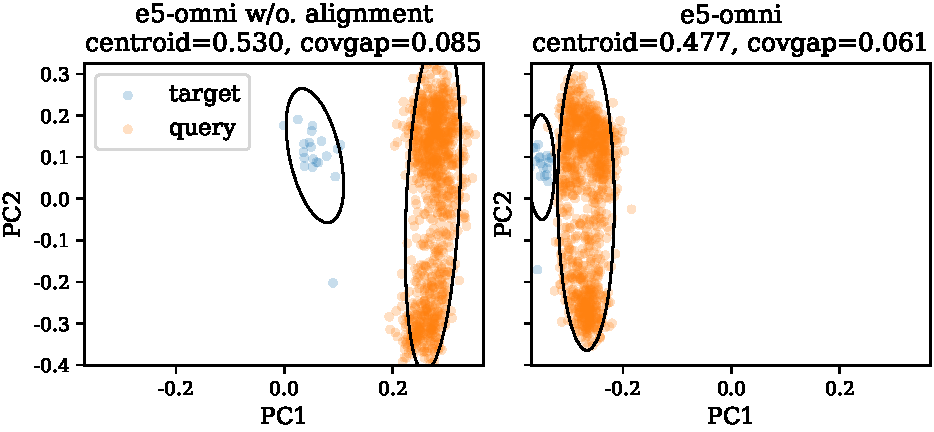
\includegraphics[width=0.98\columnwidth]{figures/modality_overlap_VOC2007.pdf}
  \caption{{PCA overlap on VOC2007.}
Left: \ours{} w/o.\ alignment. Right: \ours{}.
We project embeddings into a shared 2D PCA space and overlay $2\sigma$ covariance ellipses.
We report \emph{centroid} (distance between the query/target mean embeddings) and \emph{covgap} (Frobenius gap between their covariance matrices).}\label{fig:align-pca-voc}
\end{figure}

\paragraph{Results and interpretation.}
Compared to \ours{}~w/o.\ alignment, the full \ours{} yields smaller query--target mismatch in embedding space: the centroid gap and the covariance gap decrease in Fig.~\ref{fig:align-pca-voc}.
The covariance-difference heatmap in Fig.~\ref{fig:align-covdiff-voc} further indicates reduced second-order discrepancy with fewer high-magnitude entries.
While the heatmap mainly reflects second-order geometry (most directly tied to whitening/covariance regularization), the PCA overlap reflects both first- and second-order effects and may also be influenced by training dynamics (\eg, modality-aware logit calibration and more stable negative supervision).
Overall, these diagnostics provide distribution-level evidence that the \emph{combined} design of \ours{} promotes a more consistent shared embedding space, complementing the benchmark results.






\begin{figure}[t]
  \centering
  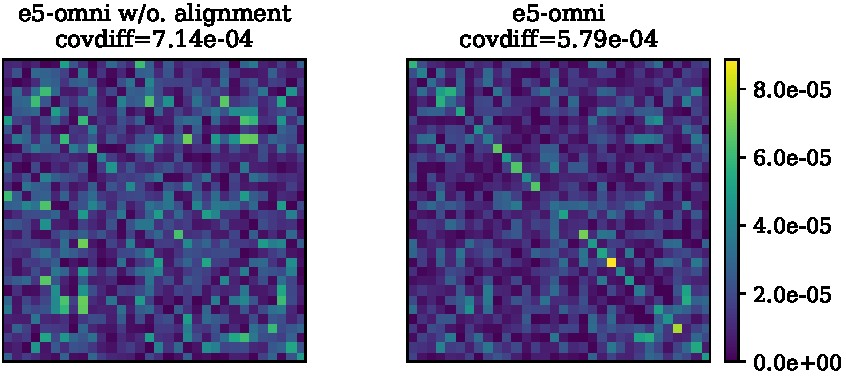
\includegraphics[width=0.98\columnwidth]{figures/covdiff_heatmap_VOC2007.pdf}
  \caption{{Covariance-difference heatmap on VOC2007.}
Left: \ours{} w/o.\ alignment. Right: \ours{}.
After a fixed 32D random projection, we visualize \emph{covdiff}: the entrywise magnitude of the query--target covariance difference matrix.}\label{fig:align-covdiff-voc}
\end{figure}

%
\subsection{Hyperparameter Analysis}
\label{subsec:param}

We analyze the sensitivity of \ours{} to key hyperparameters in our explicit alignment recipe.
We tune these hyperparameters on 1K-sample validation splits drawn from the corresponding training sets.
For consistency with prior experiments, we report results on the MMEB-V2 test sets in Fig.~\ref{fig:param}.
Additional studies are deferred to Appendix~\ref{app:param}.

\noindent\textbf{Modality-aware temperature initialization.}
Our modality-aware calibration introduces a trainable per-modality scaling vector
$\boldsymbol{\tau}$ (Sec.~\ref{subsec:method-modaltemp}).
We sweep the initialization value $\tau_0$ (\ie, initializing all entries of $\boldsymbol{\tau}$ to the same constant $\tau_0$).
We observe a trade-off: overly small $\tau_0$ yields overly sharp logits early in training, while large $\tau_0$ produces overly flat logits and slows convergence.
Overall, initializing $\boldsymbol{\tau}$ in a small range (\eg, $\tau_0\in[0.015,0.03]$) is robust, and we use $\tau_0=0.02$ by default.

\noindent\textbf{DCL debiasing coefficient.}
We sweep the DCL parameter $\gamma_{+}$ (Sec.~\ref{subsec:method-hns}), which controls the strength of debiasing under negative selection.
Moderate values work best: too small $\gamma_{+}$ provides limited correction, while too large $\gamma_{+}$ can over-correct and weaken supervision.
In our experiments, $\gamma_{+}\in[0.1,0.2]$ yields consistent improvements on MMEB-V2, and we use $\gamma_{+}=0.1$ by default.

\begin{figure}[t]
\centering
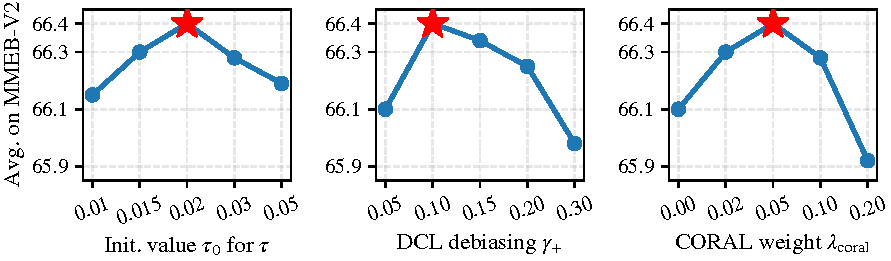
\includegraphics[width=0.5\textwidth]{figures/param_sweep.pdf}
\caption{The performances of \ours{}-7B under different training settings on MMEB-V2. We report the overall scores using same metric as in Table~\ref{tab:mmeb-v2-overall}.}\label{fig:param} 
\end{figure}

\noindent\textbf{Covariance regularization weight.}
Finally, we vary the CORAL weight $\lambda_{\mathrm{coral}}$ (Sec.~\ref{subsec:method-align}).
Increasing $\lambda_{\mathrm{coral}}$ generally improves cross-modal geometric consistency, but overly large weights can interfere with the retrieval objective.
We observe that a small auxiliary weight (\eg, $\lambda_{\mathrm{coral}}\in[0.02,0.1]$) provides the best trade-off.





\subsection{Generalization to Other VLM Backbones}
\label{subsec:generalization}

To validate that \ours{} is not tied to a specific backbone, we apply our explicit alignment recipe to multiple off-the-shelf VLMs with different sizes and architectures.
For each backbone, we first train a strong baseline w/o.\ alignment (as defined in Sec.~\ref{subsec:exp-align-viz}), and then train the full \ours{} by enabling all three techniques.

We report results on MMEB-V2 in Table~\ref{tab:generalization}.
We omit AudioCaps because only a limited number of public VLM backbones support audio inputs out of the box, making a broad backbone comparison infeasible.
Overall, \ours{} consistently improves over the corresponding baselines across all backbones, demonstrating that our method is a plug-and-play strategy for turning diverse VLM backbones into robust omni-modal embedding models.




